\documentclass{article}
\usepackage{graphicx}
\usepackage{titlepic}
\title{Sistema experto para diagnóstico de enfermedades}
\author{Molina Prieto, Francisco Javier
        \and
        Prieto Barón, Álvaro (49506913B)}
\titlepic{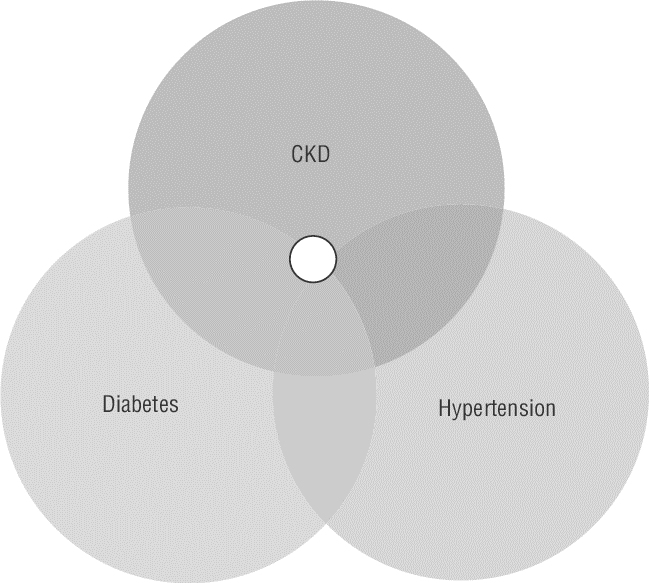
\includegraphics[width=\textwidth]{imagenportada.png}}

\begin{document}
    \maketitle
    \pagebreak
    \tableofcontents
    \pagebreak

    \section{Descripción del problema}
    \paragraph{La medicina,}
    a pesar de ser un campo muy amplío, puede ser un campo clasificado si se tiene una base de datos consistente y un Sistema que se ayude de esta para sacar conclusiones sobre, por ejemplo, qué enfermedad padece un paciente que sufre determinados síntomas. Este sistema debe indicar el nombre de la enfermedad o enfermedades que más se acercan al objetivo dados los síntomas de un enfermo.
    \paragraph{}
    Este problema en particular tiene una dificultad mayor a otros problemas de diagnóstico, dado que:
    \begin{enumerate}
        \item La proporción de síntomas respecto a enfermedades es alta, y debemos reflejar esto en nuestros datos.
        \item Es difícil que se de únicamente la totalidad de los síntomas de una enfermedad, por lo que el sistema de diagnóstico debe tener en cuenta que pueden darse síntomas extra o no darse todos.
    \end{enumerate}
    \pagebreak
    \section{Análisis del problema}
    \paragraph{}
    Para realizar este Sistema, necesitaríamos una base de datos de enfermedades y sus síntomas diferenciadores o menos comunes. Consideraremos en nuestro caso, 14 síntomas y 15 enfermedades. Podemos apreciar aquí la proporción ya mencionada en la sección anterior.
    \paragraph{}
    La tabla completa de la lista de enfermedades con sus síntomas es la siguiente:
    \paragraph{}
    \begin{tabular}{|c|l|}
    \hline
    Alergia & Lagrimeo, Estornudos
    \\ \hline
    Asma & Dificultad respiratoria, Tos
    \\ \hline
    Diabetes & Hambre, Fatiga
    \\ \hline
    Herpes & Ardor área genital, Úlceras, Fiebre, Dolor de cabeza
    \\ \hline
    Hepatitis & Fatiga, Fiebre, Náuseas
    \\ \hline
    Gastroenteritis & Fatiga, Fiebre, Dolor de cabeza, Náuseas
    \\ \hline
    Otitis & Fiebre, Dolor de oído
    \\ \hline
    Bronquitis & Fiebre, Fatiga Dificultad respiratoria
    \\ \hline
    Gripe & Fatiga, Estornudos, Tos, Congestión nasal
    \\ \hline
    Conjuntivitis & Lagrimeo, Ardor en los ojos
    \\ \hline
    Resfriado & Tos, Estornudos, Congestión nasal
    \\ \hline
    Sinusitis & Fiebre, Congestión nasal, Dolor de cabeza
    \\ \hline
    Faringitis & Dolor de oído, Fiebre, Dolor al deglutir
    \\ \hline
    Bronquiolitis & Tos, Fatiga, Fiebre, Dificultad respiratoria 
    \\ \hline
    Intoxicación & Náuseas, Fatiga, Fiebre
    \\ \hline
        
    \end{tabular}
    \paragraph{}
    Tomaremos pues estos datos y los introduciremos en nuestro sistema, que tendrá la siguiente estructura:
    \begin{itemize}
        \item Plantilla enfermedad, con 4 slots: nombre, síntomas (multislot), probabilidad de enfermedad y un campo de control.
        \item Base de datos de enfermedades (hechos basados en la plantilla anterior).
        \item Lista de síntomas.
    \end{itemize}
    \pagebreak
    \section{Funcionamiento del sistema y manual}
    \subsection{Funcionamiento del sistema}
    El sistema aceptará como entrada los síntomas del paciente y tendrá como salida las 3 enfermedades más probables que puede padecer este.
    \paragraph{}
    Cada síntoma introducido, se “confirmará” en las enfermedades en las que esté presente este.
    \paragraph{}
    Una vez introducidos todos los síntomas, se comprobará el total de síntomas confirmados de cada enfermedad (con la longitud del slot \emph{symptoms} antes mencionado) y se dividirá entre el número total de síntomas de esta, obteniendo así la probabilidad de que esta sea la enfermedad que padece el paciente.
    \paragraph{}
    Este sistema tiene este funcionamiento debido a que no todas las enfermedades tienen síntomas únicos o el mismo número total de síntomas, por lo que es el modo más preciso para clasificarlas.
    \subsection{Manual de usuario}
    \paragraph{}
    Lo primero que debe hacer el usuario es iniciar CLIPS y cargar el programa. Tras hacer \emph{(reset)} y ejecutar, aparecerá un menú con 4 opciones:
    \begin{itemize}
        \item 0. Salir
        \item 1. Añadir síntoma
        \item 2. Eliminar último síntoma añadido
        \item 3. Mostrar resultado del diagnóstico
    \end{itemize}
    \paragraph{}
    Los síntomas deben ser añadidos como cadenas (es decir, entre ""), y en minúscula, de forma que el sistema pueda reconocerlos.
    \paragraph{}
    Tras pulsar la opción 3, el sistema calculará la probabilidad de cada enfermedad y mostrará las 3 más altas.
    \pagebreak
    \section{Equipo de desarrollo} 
    \paragraph{}
    El equipo está formado por:
    \begin{itemize}
        \item Álvaro Prieto Barón: Encargado del backend y la analítica del sistema. Iniciador de la idea del funcionamiento del sistema para el análisis estadístico de enfermedades. Documentación sobre el funcionamiento del sistema.
        \item Fco. Javier Molina Prieto: Encargado de la base de datos del sistema y de la documentación del análisis y descripción del problema. 
    \end{itemize}

\end{document} 